\documentclass[landscape,10pt]{beamer}
\usepackage{graphicx}
\usepackage{color}
\usepackage{bm}
\usepackage{ulem}
\usepackage[backend=bibtex,natbib, citestyle=authoryear]{biblatex}
\usepackage{listings}
\addbibresource{/home/qungibbo/docs/references/notes}
\renewcommand*{\bibfont}{\tiny}

\newcommand*{\mathcolour}{}
\def\mathcolour#1#{\mathcoloraux{#1}}
\newcommand*{\mathcoloraux}[3]{%
\protect\leavevmode
\begingroup
\color#1{#2}#3%
\endgroup
}

\lstset{language=Python,
                basicstyle=\ttfamily,
                keywordstyle=\color{blue}\ttfamily,
                stringstyle=\color{red}\ttfamily,
                commentstyle=\color{gray}\ttfamily,
                morecomment=[l][\color{magenta}]{\#}
}

\newcommand{\stkout}[1]{\ifmmode\text{\sout{\ensuremath{#1}}}\else\sout{#1}\fi}
\lstset{basicstyle=\ttfamily}
\usecolortheme{dove}
\beamertemplatenavigationsymbolsempty
\setbeamertemplate{caption}[numbered]
\setbeamertemplate{bibliography item}{}

\usefonttheme[onlymath]{serif}
%\renewcommand{\familydefault}{\rmdefault}
\makeatletter
\def\input@path{{./images/}}
\makeatother
\newcommand{\svginput}[1]{\input{#1}} 
\graphicspath{{./images/}}
\renewcommand{\footnotesize}{\tiny}

\title{\textbf{Scientific Programming: Miscellaneous tricks, tips and lessons learned}}

 \author{
  Nick N. Gibbons,\\
  {\itshape
   The University of Queensland, Brisbane, Queensland 4072, Australia}\\
 }

\begin{document}
\frame{\titlepage}

\begin{frame}
\frametitle{Outline: Scientific Computing Group Seminar}
\vspace{5mm}
\begin{itemize}
\item Linux Core Dev Toolkit
\begin{itemize}
\item grep
\item The Editor Wars
\item history searching
\item rsync
\end{itemize}
\item Advanced Paraview
\begin{itemize}
\item Programmable Filters
\item Scripting interface
\end{itemize}
\item numpy
\begin{itemize}
\item ndarrays
\item logical operations
\item einsum
\item linear algebra
\end{itemize}
\item Embedding C code in Python
\begin{itemize}
\item A simple example: Particle Motion
\item A complicated example: Vortex Visualisation
\end{itemize}
\end{itemize}
\end{frame}

\begin{frame}[fragile]
\frametitle{Linux Core Dev Toolkit: grep}
\begin{itemize}
\item Search text, count things, evaluate regular expressions
\end{itemize}

\begin{verbatim}
$ cat *.log | grep -c grep | awk '{ print $1/1035 }' 
4.61256
\end{verbatim}

\begin{itemize}
\item Normal Usage: 
\end{itemize}
\begin{scriptsize}
\begin{verbatim}
$ grep with_k_omega *.d
    shape_sensitivity_calc.d: //if (with_k_omega) nPrimitive += 2;
\end{verbatim}
\end{scriptsize}

\begin{itemize}
\item Recursive Usage: 
\end{itemize}
\begin{scriptsize}
\begin{verbatim}
$ grep -r with_k_omega --include="*.d"
    fvcell.d:    bool allow_k_omega_update = true;
    bc/boundary_cell_effect.d:        blk.get_cell(i,j,k)
                   .allow_k_omega_update = false;
\end{verbatim}
\end{scriptsize}

\begin{itemize}
\item Find repeated words with a regular expression:
\end{itemize}
\begin{verbatim}
$ grep -E "\b([a-zA-Z]+) \1\b" words.txt
\end{verbatim}
\end{frame}

\begin{frame}[fragile]
\frametitle{Linux Core Dev Toolkit: The Editor Wars}
\begin{figure}[h]
    \centering
    
\includegraphics[width=0.70\textwidth]{texteditors.png}
\end{figure}

\begin{itemize}
\item ViM: (Vi Improved)
\begin{itemize}
\item Pros: Powerful, runs on everything, very configurable
\item Cons: Steep learning curve, hard to quit 
\end{itemize}
\end{itemize}

\begin{itemize}
\item EMACS: (Exclusively used by Middle Aged Computer Scientists)
\begin{itemize}
\item Pros: More intuitive than vim, also powerful and configurable
\item Cons: Also steep learning curve, destroyer of alt/ctrl/shift keys
\end{itemize}
\end{itemize}

\begin{itemize}
\item Sublime Text:
\begin{itemize}
\item Pros: Feature packed, easy to use, looks nice
\item Cons: Closed source, (winzip style?)
\end{itemize}
\end{itemize}

\begin{itemize}
\item Others: Atom/Nano/etc.
\end{itemize}

\end{frame}

\begin{frame}[fragile]
\frametitle{Linux Core Dev Toolkit: History Searching}
\begin{itemize}
\item Commands typed into the linux commandline are saved in \texttt{.bash\_history}
\item \texttt{.inputrc} can be configured to search through these while typing
\end{itemize}

\begin{verbatim}
$ make_
$ make INSTALL_DIR=/home/nick/programs/dgd/dmd install_
\end{verbatim}

\begin{itemize}
\item Specific commands for UP and DOWN to search are:
\end{itemize}
\begin{verbatim}
"\e[A": history-search-backward
"\e[B": history-search-forward
\end{verbatim}

\begin{itemize}
\item This automatically works with other programs that use libreadline
\begin{itemize}
\item ipython3 etc.
\end{itemize}
\end{itemize}

\end{frame}

\begin{frame}[fragile]
\frametitle{Linux Core Dev Toolkit: rsync}
\begin{itemize}
\item rsync is a powerful file copying utility
\item Use 1: Copy things to another computer over ssh
\item Use 2: archiving data (with -tarvPp)
\end{itemize}
 
\begin{scriptsize}
\begin{verbatim}
rsync -tarvPp --delete /home/qungibbo/ /media/qungibbo/Elements/
WintermuteSSD --exclude "*.ssh" --exclude "programs/*"
--exclude "sourcecode/us3d*" --exclude "sourcecode/paraview*"
--exclude "sourcecode/cfcfd3/*" --exclude "sourcecode/hdf5-1.8.12/*"
--exclude "sourcecode/openmpi-1.8.12/*" --exclude "*.vtk"
--exclude "*.o" --exclude "*.mod" --exclude ".cache*"
--exclude ".wine/*" --exclude "*.swp" --exclude "*.pvtu"
--exclude "*.vtu" --exclude "*.npy"

rsync -tarvPp --delete /media/qungibbo/data/ /media/qungibbo/Elements/
WintermuteDATA --exclude "binaries/*" --exclude "*.vtk" --exclude "*.o"
--exclude   "*.mod" --exclude "*.swp" --exclude "*.pvtu"
--exclude "*.vtu" --exclude "*.npy"
\end{verbatim}
\end{scriptsize}

\end{frame}

\begin{frame}[fragile]
\frametitle{Advanced Post Processing: Paraview Programmable Filters}
\begin{itemize}
\item Paraview workflow uses "Filters" to process data
\item Common Filters: Slice, Gradients, Calculator
\item "Programmable Filter" is a custom filter that uses a python script to do anything
\item "Can I do-" "Yes"
\end{itemize}

\vspace{10mm}

Example to compute vorticity vector:
\begin{scriptsize}
\begin{lstlisting}
du = zeros((neq,neq,nx)) # du[i,j] = du_i / dx_j
du[0] = algs.gradient(u).T
du[1] = algs.gradient(v).T
du[2] = algs.gradient(w).T

vort = zeros((neq,nx))
vort[0] = du[2,1] - du[1,2]
vort[1] = du[0,2] - du[2,0]
vort[2] = du[1,0] - du[0,1]
\end{lstlisting}
\end{scriptsize}

\end{frame}

\begin{frame}[fragile]
\frametitle{Advanced Post Processing: Paraview Programmable Filters}
\begin{itemize}
\item More complicated example: Mixing Efficiency
\end{itemize}

\begin{scriptsize}
\begin{lstlisting}
splist = "N2,O2,H2,H2O,OH,HO2,H2O2,NO,NO2,HNO,N,H,O".split(',')
gassp = {n:get_species(n) for n in splist}
rhos = [get_array('r{}m'.format(i+1)) for i in range(len(splist))]
rho = sum(rhoi for rhoi in rhos)
cs  = [rhoi/rho for rhoi in rhos]

# Compute the fraction of mass of each atom made up by H or O, excluding anything   involving N
atomicmass = lambda s,atom : sum(gassp[k].M*v for k,v in gassp[s].atoms.items() if  k==atom)
mH =[0.0 if 'N' in s else atomicmass(s,'H')/gassp[s].M for s in splist]
mO =[0.0 if 'N' in s else atomicmass(s,'O')/gassp[s].M for s in splist]
YO = sum(mOi*csi for mOi,csi in zip(mO, cs))
YH = sum(mHi*csi for mHi,csi in zip(mH, cs))

Ytotal = YO + YH # Mass fraction of the flow that is interesting from a mixing perspective
YYH = YH/Ytotal  # Mass fraction fraction of the interesting flow that is Hydrogen atoms
YYO = YO/Ytotal  # Mass fraction fraction of the interesting flow that is Oxygen atoms
massst = 0.5*gassp['O2'].M/(1.0*gassp['H2'].M) # Stoichiometric Oxygen/hydrogen mass ratio

# Fraction of interesting flow fraction that is mixed
YYmixed = np.minimum(YYH*(1.0 + massst), YYO*(1.0 + 1.0/massst))
\end{lstlisting}
\end{scriptsize}
\end{frame}

\begin{frame}[fragile]
\frametitle{Advanced Post Processing: Paraview Scripting}
\begin{itemize}
\item Paraview has an extremely flexible python scripting interface
\item You can automate ANYTHING
\item Click "Start Trace" in "Tools", do something, then "Stop Trace"
\end{itemize}

\begin{scriptsize}
\begin{lstlisting}
from paraview.simple import *
from glob import glob
from sys import argv

scriptname = argv[1]
pattern = argv[2]
files = glob(pattern)
files.sort()

with open(scriptname) as fp:
     script = fp.read()

for i,filename in enumerate(files):
    print "Computing file: ", filename, scriptname

    soln = OpenDataFile(filename)
    prgfil = ProgrammableFilter(soln)
    my_script = script.replace('REPLACE',str(i).zfill(3))
    prgfil.Script = my_script

    Show(prgfil)
    Delete(prgfil)
    Delete(soln)
\end{lstlisting}
\end{scriptsize}
\end{frame}

\begin{frame}[fragile]
\frametitle{numpy: Fast numerical computation in python}
\begin{itemize}
\item numpy is core utility library for numerical computation in python
\item ndarray objects are extremely powerful but can be confusing at first
\item Their main use is looping without using very slow interpreted "for" loops
\end{itemize}

\vspace{7mm}
\begin{small}
\begin{lstlisting}
In[9]: %timeit for i in range(1000): c[i] = a[i]*c[i]
10000 loops, best of 3: 122 us per loop
\end{lstlisting}
\end{small}

\begin{small}
\begin{lstlisting}
In[13]: %timeit c = a*b
1000000 loops, best of 3: 1.06 us per loop
\end{lstlisting}
\end{small}

\end{frame}

\begin{frame}[fragile]
\frametitle{numpy: Tips and tricks}
\begin{itemize}
\item Vectorisation Example: Logic
\item Copy the smaller element to array c
\end{itemize}

\begin{scriptsize}
\begin{lstlisting}
a = random.random(1000)
b = random.random(1000)

# Slow:
c = []
for i,j in a,b:
    if i<j:
        c.append(i)
    else:
        c.append(j)

# Fast
d = a<b           # bool array of true falses
c = d*a + (1-d)*b # acts like 1 or zero in arithmatic
\end{lstlisting}
\end{scriptsize}

\end{frame}

\begin{frame}[fragile]
\frametitle{numpy: Tips and tricks}
\begin{itemize}
\item Vectorisation Example: Matrix Multiplication
\item Matrix multiply a large number of matching matrices with einsum
\end{itemize}

\begin{scriptsize}
\begin{lstlisting}
A = random.random(100*3*3).reshape((100,3,3))
B = random.random(100*3*3).reshape((100,3,3))

# Slow:
C = []
for i in A.shape[0]:
    C.append(A[i].dot(B[i])

# Fast
C = einsum('lij,ljk->lik', A, B)
\end{lstlisting}
\end{scriptsize}

\end{frame}

\begin{frame}[fragile]
\frametitle{numpy: Tips and tricks}
\begin{itemize}
\item Vectorisation Example: Linear Algebra
\item Solve a large number of algebra problems
\end{itemize}

\begin{scriptsize}
\begin{lstlisting}
from numpy.linalg import eig
A = random.random(100*3*3).reshape((100,3,3))

# Slow:
evals = []
evecs = []
for i in A.shape[0]:
    eval,evec  = eig(A[i])
    evals.append(eval)
    evecs.append(evecs)

# Fast
evals, evecs = eig(A)
\end{lstlisting}
\end{scriptsize}

\end{frame}

\begin{frame}[fragile]
\frametitle{numpy: Tips and tricks}
\begin{itemize}
\item Always check the library functions!
\item If you need it chances are someone else has too
\item Vectorisation Example: binning data for a histogram
\end{itemize}

\begin{scriptsize}
\begin{lstlisting}
>>> x = np.array([0.2, 6.4, 3.0, 1.6])
>>> bins = np.array([0.0, 1.0, 2.5, 4.0, 10.0])
>>> inds = np.digitize(x, bins)
>>> inds
array([1, 4, 3, 2])
>>> for n in range(x.size):
...   print(bins[inds[n]-1], "<=", x[n], "<", bins[inds[n]])
...
0.0 <= 0.2 < 1.0
4.0 <= 6.4 < 10.0
2.5 <= 3.0 < 4.0
1.0 <= 1.6 < 2.5
\end{lstlisting}
\end{scriptsize}

\end{frame}

\begin{frame}[fragile]
\frametitle{Coupling C code with Python}
\begin{itemize}
\item What to do when your application really is too complex for numpy
\item Python builtin library ctypes allows you call c code from python
\item Simple Example: Integrating Particle Motion
\item Complicated Example: The Triple Decomposition Method
\end{itemize}

\end{frame}

\begin{frame}[fragile]
\frametitle{Coupling C code with Python: Particle Motion}
Pure Python Implementation of a Falling Particle:
\begin{scriptsize}
\begin{lstlisting}
dt = 0.0001
N = 61500
x  = array([0.0, 0.0])
xd = array([30.0, 30.0])
xdd= array([0.0, -9.81])
xs = zeros((N,2))

start = time.clock()
for i in range(N):
    x += xd*dt + 0.5*xdd*dt**2
    xd += xdd*dt
    xs[i] = x.copy()

end = time.clock()
print("Time for N={}: {:4.4f}ms".format(N, (end-start)*1000.0))
\end{lstlisting}
\end{scriptsize}

\end{frame}

\begin{frame}[fragile]
\frametitle{Coupling C code with Python: Particle Motion}
Pure Python Implementation of a Falling Particle:

\begin{figure}[h]
    \tiny
    \centering
    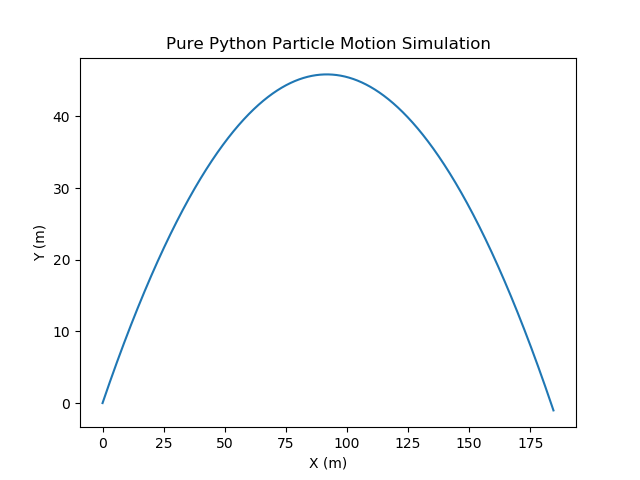
\includegraphics[width=0.90\textwidth]{pyshot_particle.png}
\end{figure}
\end{frame}

\begin{frame}[fragile]
\frametitle{Coupling C code with Python: Particle Motion}
Hybrid Implementation of a Falling Particle: Python Side
\begin{scriptsize}
\begin{lstlisting}
dt = 0.0001
N = 61500
x  = array([0.0, 0.0])
xd = array([30.0, 30.0])
xdd= array([0.0, -9.81])
xs = zeros((N,2))

c_double_p = POINTER(c_double)
xp = x.ctypes.data_as(c_double_p)
xdp = xd.ctypes.data_as(c_double_p)
xddp = xdd.ctypes.data_as(c_double_p)
xsp = xs.ctypes.data_as(c_double_p)
dt_c = c_double(dt)
lib = cdll.LoadLibrary('libodeint.so')

start = time.clock()
lib.integrate_particle(xp, xdp, xddp, xsp, N, 2, dt_c)
end = time.clock()

print("Time for N={}: {:4.4f}ms".format(N, (end-start)*1000.0))
\end{lstlisting}
\end{scriptsize}

\end{frame}

\begin{frame}[fragile]
\frametitle{Coupling C code with Python: Particle Motion}
Hybrid Implementation of a Falling Particle: C side
\begin{scriptsize}
\begin{lstlisting}[language=C]
void integrate_particle(double* x, double* xd, double* xdd, double* xs,
                        int N, int  dim, double dt){
    // Simple fixed timestep integrator
    for(int i=0; i<N; i++) {
        for(int d=0; d<dim; d++) {
            x[d] += xd[d]*dt + 0.5*xdd[d]*dt*dt;
            xd[d] += xdd[d]*dt;
            xs[i*dim + d] = x[d];
        }
    }
    return;
}
\end{lstlisting}
\end{scriptsize}
Compare the Python Loop:
\begin{scriptsize}
\begin{lstlisting}
for i in range(N):
    x += xd*dt + 0.5*xdd*dt**2
    xd += xdd*dt
    xs[i] = x.copy()
\end{lstlisting}
\end{scriptsize}

\end{frame}

\begin{frame}[fragile]
\frametitle{Coupling C code with Python: Particle Motion}
Compiling C code into a dynamic library:
\begin{verbatim}
$ gcc -c -fPIC odeint.c
$ gcc -shared odeint.o -o libodeint.so
\end{verbatim}

Speedup is significant:
\begin{verbatim}
nick@spark:~/code/randomcrap$ python3 pyshot.py
Time for N=61500: 461.6890ms

nick@spark:~/code/randomcrap$ python3 cshot.py
Time for N=61500: 1.2420ms
\end{verbatim}
\end{frame}

\begin{frame}[fragile]
\frametitle{Coupling C code with Python: Vortex Visualisation}
\begin{itemize}
\item There are many vortex visualisation techniques that use the decomposed velocity gradients:
\end{itemize}

%\begin{equation}
%\frac{\partial u_i}{\partial u_j} = S_{ij} + \Omega_{ij}
%\end{equation}

%\begin{equation}
%S_{ij} = \frac{1}{2} \left[\frac{\partial u_i}{\partial x_j} + \frac{\partial u_j}{\partial x_i} \right] ~~~ \Omega_{ij} = \frac{1}{2} \left[\frac{\partial u_i}{\partial x_j} - \frac{\partial u_j}{\partial x_i} \right]
%\end{equation}

\begin{figure}[h]
    \tiny
    \centering
    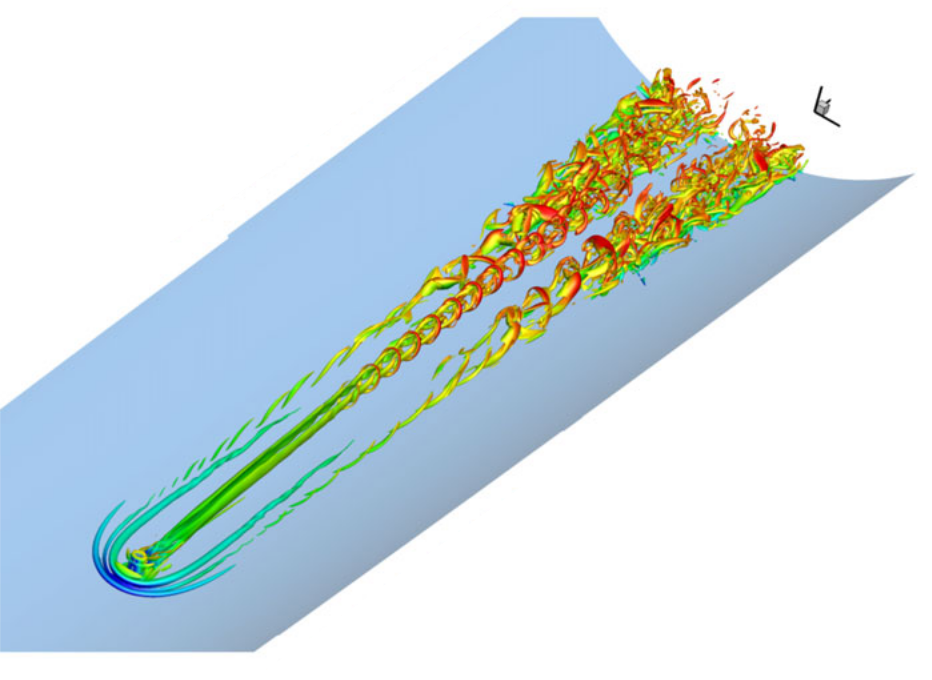
\includegraphics[width=0.80\textwidth]{candler_fig9b.png}
    \caption{Vortex visualisation using the Q criterion, from Subbareddy, Bartkowicz, and Candler (2015), figure 9} 
    \label{candler_fig9b}
\end{figure}

\end{frame}

\begin{frame}[fragile]
\frametitle{Coupling C code with Python: Vortex Visualisation}
\begin{itemize}
\item In subsonic flow this is pretty straightforward, first compute $S$ and $\Omega$
\end{itemize}

\begin{equation}
\frac{\partial u_i}{\partial u_j} = S_{ij} + \Omega_{ij}
\end{equation}

\begin{equation}
S_{ij} = \frac{1}{2} \left[\frac{\partial u_i}{\partial x_j} + \frac{\partial u_j}{\partial x_i} \right] ~~~ \Omega_{ij} = \frac{1}{2} \left[\frac{\partial u_i}{\partial x_j} - \frac{\partial u_j}{\partial x_i} \right]
\end{equation}

\begin{itemize}
\item Then pick a vortex identification method, eg:
\begin{itemize}
\item Q criterion: $Q = \frac{1}{2}(||\Omega||^2 - ||S||^2) > 0$
\vspace{2mm}
\item $\Delta$-criterion: $(Q/3)^3 + (det(\nabla u)/2)^2 > 0$
\vspace{2mm}
\item $\lambda_2$ method: $eigvals(\Omega^2 + S^2) = \lambda_1, \lambda_2, \lambda_3 ~~~ : ~~~ \lambda_2 < 0$
\vspace{2mm}
\end{itemize}
\end{itemize}

\end{frame}

\begin{frame}[fragile]
\frametitle{Coupling C code with Python: Vortex Visualisation}
\begin{itemize}
\item In supersonic flow these can be cluttered with shockwaves since the shearing motion is incorrectly included as if it were a vortex
\item The Triple Decomposition Method subtracts out a pure shearing term:
\end{itemize}

\begin{equation}
\frac{\partial u_i}{\partial u_j} - \left(\frac{\partial u_i}{\partial u_j}\right)_{SH} = S_{ij}^{TDM} + \Omega_{ij}^{TDM}
\end{equation}

\begin{itemize}
\item Once $\left(\nabla u\right)_{SH}$ is found plug $S_{ij}^{TDM} + \Omega_{ij}^{TDM}$ into your vortex identification method
\item How to compute $\left(\nabla u\right)_{SH}$ ?
\end{itemize}
\end{frame}

\begin{frame}[fragile]
\frametitle{Coupling C code with Python: Vortex Visualisation}
\begin{itemize}
\item Computing $\left(\nabla u\right)_{SH}$ requires a nasty optimisation problem in every cell
\item Rotate the axes $\nabla u \rightarrow \nabla u'$ and find the angles where:
\end{itemize}
\begin{equation}
MAX(|S_{12}'\Omega_{12}'| + |S_{23}'\Omega_{23}'| + |S_{31}'\Omega_{31}'|)
\end{equation}

\begin{itemize}
\item In this reference frame it is possible to compute $(\nabla u)_{SH}$
\item Then subtract out $S_{ij}^{TDM} + \Omega_{ij}^{TDM}$ and convert back into lab frame
\end{itemize}

\end{frame}

\begin{frame}[fragile]
\frametitle{Coupling C code with Python: Vortex Visualisation}
\begin{itemize}
\item Pure python implementation is EXTREMELY SLOW ($\approx 30$ hours to execute)
\item Instead call a C routine from inside Paraview to do the same thing 
\item This takes $\approx 20$ mins or so, and can be done in parallel
\end{itemize}

\end{frame}

\begin{frame}[fragile]
\frametitle{Coupling C code with Python: Vortex Visualisation}
\begin{figure}[h]
    \scriptsize
    \centering
    \def\svgwidth{0.99\columnwidth}
    \svginput{vort_flipped.pdf_tex}
    \caption{Vortex visualisation using TDM and the L2 method with pressure colour maps.}
    \label{vort_flipped}
\end{figure}

\end{frame}


\begin{frame}[fragile]
\frametitle{Conclusions}
\begin{itemize}
\item Command line tools are very powerful, learn to use them!
\item Get comfortable with a good text editor
\item Interpreted languages (Python,R) are great for scientific computing
\begin{itemize}
\item As long as you use the datastructures properly!
\item Both python and R come packed with builtin functions too
\end{itemize}
\item If you need to fall back on some low-level programming, (C etc.) tools exist to integrate them into higher level languages.
\end{itemize}

%\begin{scriptsize}
%\begin{lstlisting}
%\end{lstlisting}
%\end{scriptsize}

\end{frame}


%\frametitle{References}
%\end{frame}


\end{document}
